\documentclass{standalone}

\usepackage{tikz}

\usetikzlibrary{arrows}
\usetikzlibrary{calc}



\begin{document}

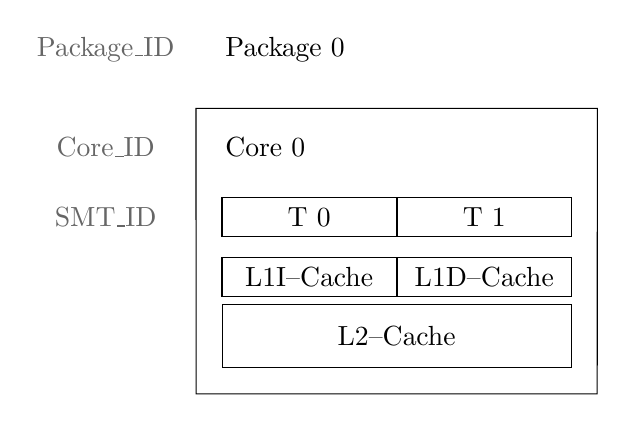
\begin{tikzpicture}[node distance=5mm, scale=2]

  % Colors
  % Styles
  \tikzstyle{package_style} = 
    [font=\normalsize, text top left, text width=2cm, draw=black, shape=rectangle, inner sep = 1pt]
  \tikzstyle{thread_style} = 
    [font=\normalsize, text centered, text width=2cm, draw=black,
    shape=rectangle, inner sep = 3pt, minimum width = 1cm, minimum height =.5cm]

  \tikzstyle{id_style} = [font=\normalsize, text centered, draw=none,
  color=black!60!white, rectangle]

  \tikzstyle{thread_shape} = \draw[thread_style];
  \tikzstyle{l1_cache_shape} = \draw[thread_style];
  \tikzstyle{l2_cache_shape} = [thread_style, minimum width = 4.43cm, minimum
    height =.8cm];

  % Drawing

  % First core
    \node(l2)	[l2_cache_shape] {L2--Cache};
    \node(l1i)  [l1_cache_shape, above of=l2, anchor=south east] {L1I--Cache};
    \node(l1d)  [l1_cache_shape, above of=l2, anchor=south west] {L1D--Cache};

    \node(t0)	[thread_shape, above of=l1i, anchor=south] {T 0};
    \node(t1)	[thread_shape, above of=l1d, anchor=south] {T 1};

    \draw [transparent] (l2.south west) -- ++(-1mm,-1mm) node(swc) {};
    \draw [transparent] (l2.south east) -- ++(1mm,-1mm) node(sec) {};
    \draw [transparent] (t1.north east) -- ++(1mm,5mm) node(nec) {};
    \draw [transparent] (t0.north west) -- ++(-1mm,5mm) node(nwc) {};

    \draw[black] (swc.south west) -- (sec.south east) -- (nec.north east) --
    (nwc.north west) -- cycle;

    \node(core0) [anchor=north west] at (nwc.south east) {Core 0};

    \node(smt_id) [id_style, anchor=east, xshift=-7mm] at (t0.west) {SMT\_ID};
    \draw[transparent] (smt_id.north) |- coordinate[midway](corner) (core0.west);
    \node(core_id) [id_style] at (corner) {Core\_ID};
  

    \draw[transparent] (core0.north west) -- ++(0,5mm) coordinate(pid);
    \node(pack0) [rectangle, draw=none, anchor=west] at (pid) {Package 0};
    
    \draw[transparent] (core_id.north) |- coordinate[midway](pidc) (pid);
    \node(package_id) [id_style] at (pidc) {Package\_ID};
  % Second core


\end{tikzpicture}

\end{document}
